% !TeX spellcheck = <none>
\documentclass[11pt]{charter}
\usepackage[shortlabels]{enumitem}


% El títulos de la memoria, se usa en la carátula y se puede usar el cualquier lugar del documento con el comando \ttitle
\titulo{Sistema de sensores autónomos para monitoreo de redes de distribución de baja tensión mediante LoRaWAN} 

% Nombre del posgrado, se usa en la carátula y se puede usar el cualquier lugar del documento con el comando \degreename
\posgrado{Carrera de Especialización en Sistemas Embebidos} 
%\posgrado{Carrera de Especialización en Internet de las Cosas} 
%\posgrado{Carrera de Especialización en Intelegencia Artificial}
%\posgrado{Maestría en Sistemas Embebidos} 
%\posgrado{Maestría en Internet de las cosas}

% Tu nombre, se puede usar el cualquier lugar del documento con el comando \authorname
\autor{Ing. Milton Eduardo Sosa} 

% El nombre del director y co-director, se puede usar el cualquier lugar del documento con el comando \supname y \cosupname y \pertesupname y \pertecosupname
\director{Ing. Marcelo E. Romeo}
\pertenenciaDirector{UNSAM} 
% FIXME:NO IMPLEMENTADO EL CODIRECTOR ni su pertenencia
\codirector{} % si queda vacio no se deberíá incluir 
\pertenenciaCoDirector{}

% Nombre del cliente, quien va a aprobar los resultados del proyecto, se puede usar con el comando \clientename y \empclientename
\cliente{Ing. Marcelo E. Romeo}
\empresaCliente{Universidad Nacional de San Martín}

% Nombre y pertenencia de los jurados, se pueden usar el cualquier lugar del documento con el comando \jurunoname, \jurdosname y \jurtresname y \perteunoname, \pertedosname y \pertetresname.
\juradoUno{Nombre y Apellido (1)}
\pertenenciaJurUno{pertenencia (1)} 
\juradoDos{Nombre y Apellido (2)}
\pertenenciaJurDos{pertenencia (2)}
\juradoTres{Nombre y Apellido (3)}
\pertenenciaJurTres{pertenencia (3)}
 
\fechaINICIO{22 de junio de 2020}		%Fecha de inicio de la cursada de GdP \fechaInicioName
\fechaFINALPlanificacion{22 de Agosto de 2020} 	%Fecha de final de cursada de GdP
\fechaFINALTrabajo{22 de Diciembre de 2020}		%Fecha de defensa pública del trabajo final


\begin{document}

\maketitle
\thispagestyle{empty}
\pagebreak


\thispagestyle{empty}
{\setlength{\parskip}{0pt}
\tableofcontents{}
}
\pagebreak


\section{Registros de cambios}
\label{sec:registro}


\begin{table}[ht]
\label{tab:registro}
\centering

\begin{tabularx}{\linewidth}{@{}|c|X|c|@{}}
\hline
\rowcolor[HTML]{C0C0C0} 
Revisión & \multicolumn{1}{c|}{\cellcolor[HTML]{C0C0C0}Detalles de los cambios realizados} & Fecha      \\ \hline
1.0      & Creación del documento                                                          & 22/06/2020 \\ \hline
1.2      & Avances hasta el desglose de trabajo en tareas.                                 & 10/07/2020 \\ \hline
1.3      &  \shortstack[l]{
	Se corrigen errores ortográficos y espaciado entre párrafos. \\
	Se agranda el tamaño de las figuras 1 y 2.\\
	Marcelo E. Romeo pasa a ocupar el rol de cliente.\\
	Se corrigen los requerimientos y estimaciones del desglose del\\
	trabajo en tareas.
}
& 17/07/2020 \\ \hline
\end{tabularx}
\end{table}

\pagebreak



\section{Acta de Constitución del Proyecto}
\label{sec:acta}

\begin{flushright}
Buenos Aires, \fechaInicioName
\end{flushright}

\vspace{2cm}

Por medio de la presente se acuerda con el \authorname\hspace{1px} que su Trabajo Final de la \degreename\hspace{1px} se titulará ``\ttitle'', consistirá esencialmente en el prototipo preliminar de un sistema embebido que sea capaz de determinar valores eficaces de corriente alterna en redes de distribución de baja tensión y enviarlos a un centro de operaciones. Será no invasivo y autónomo. Tendrá un presupuesto preliminar estimado de 671 hs de trabajo y \$100.000, cien mil pesos argentinos, con fecha de inicio \fechaInicioName\hspace{1px} y fecha de presentación pública \fechaFinalName.

Se adjunta a esta acta la planificación inicial.

\vfill

% Esta parte se construye sola con la información que hayan cargado en el preámbulo del documento y no debe modificarla
\begin{table}[ht]
\centering
\begin{tabular}{ccc}
\begin{tabular}[c]{@{}c@{}}Ariel Lutenberg \\ Director posgrado FIUBA\end{tabular} &  & \begin{tabular}[c]{@{}c@{}}\clientename \\ \empclientename \end{tabular} \vspace{2.5cm} \\ 
\multicolumn{3}{c}{\begin{tabular}[c]{@{}c@{}} \supname \\ Director del Trabajo Final\end{tabular}} \vspace{2.5cm} \\
\begin{tabular}[c]{@{}c@{}}\jurunoname \\ Jurado del Trabajo Final\end{tabular}     &  & \begin{tabular}[c]{@{}c@{}}\jurdosname\\ Jurado del Trabajo Final\end{tabular}  \vspace{2.5cm}  \\
\multicolumn{3}{c}{\begin{tabular}[c]{@{}c@{}} \jurtresname\\ Jurado del Trabajo Final\end{tabular}} \vspace{.5cm}                                                                     
\end{tabular}
\end{table}




\section{Descripción técnica-conceptual del Proyecto}
\label{sec:descripcion}

%\begin{consigna}{black}
El presente trabajo surge como idea del autor, en base a la necesidad de permitir a las redes de distribución metropolitanas y megalopolitanas integrar características de las así llamadas Ciudades Inteligentes y así enmarcarlas dentro del concepto de Internet de las Cosas (IoT). Una ciudad inteligente, es aquella que hace uso de las diferentes tecnologías de información y comunicación disponibles con el objetivo de lograr su desarrollo sostenible, mejorar la calidad de vida de los ciudadanos y hacer un uso eficiente de los recursos energéticos.\\

Se siguen las premisas de minimizar impactos y costos de implementación en las redes de distribución actual y a la vez lograr un aumento en la calidad de servicio de energía eléctrica haciendo uso de los datos relevados.\\

Es menester mencionar que este trabajo es parte de un proyecto de una PyME de base tecnológica con el objeto de prestar servicios a diferentes empresas distribuidoras de energía electrica en Sudamérica, como así también a personas que deseen monitorear el estado de una carga eléctrica en particular haciendo uso de una estructura de red de comunicación de largo alcance.\\

El sistema que se propone implementar, ocuparía un mínimo espacio físico adicional en la red. Sin embargo, la información que proporcionaría sería de gran relevancia para realizar un relevamiento en tiempo semi real del estado de operación de la red de distribución de energía eléctrica.\\

Entre las características técnicas que sobresalen de este sistema se encuentra la utilización de tecnologías de comunicación de largo alcance y bajo consumo de energía, como por ejemplo LoRa y redes LoRaWAN, para reportar el estado de operación de un nodo en particular de la red. También propone el uso de formas de conversión y acumulación de energía eléctrica de bajo impacto medioambiental con el objeto de lograr autonomía de operación aún en condiciones meteorológicas desfavorables y operando en régimen 24/7.\\

Finalmente, es la intención de que este prototipo se mantenga independiente de la frecuencia y tensión de operación otorgando así, facilidad a la hora de realizar el comisionamiento en diferentes redes.\\

El sistema propuesto se compondrá por un hardware (HW) a desarrollar para cada nodo y los servicios interconectados en la nube también llamados backend services (BES).\\
\label{sec:diagrama_de_bloques_HW}\\
El diagrama de bloques del HW a desarrollar es presentado en la Figura \ref{fig:diagBloques}. Este posee cinco etapas:
\vspace{25px}
\begin{figure}[H]
	\centering 
	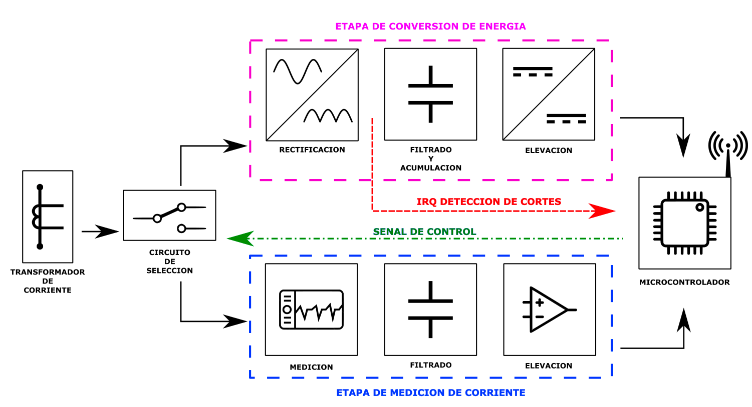
\includegraphics[width=\textwidth]{./Figuras/HW_block_diagram.png}
	\caption{Diagrama en bloques del hardware asociado al sistema.}
	\label{fig:diagBloques}
\end{figure}
\vspace{15px}
\begin{itemize}
	\item Transformador de corriente (TI): encargado de proveer de corriente eléctrica para la carga del acumulador, como así también actuar como  transductor de corriente para la medición de su valor eficaz.\\

	\item Etapa de conversión y acumulación de energía: compuesta por un rectificador de baja caída, un acumulador y un conversor DC/DC.\\

	\item Etapa de medición/detección de corriente: encargado de las mediciones de valor eficaz de corriente alterna junto a un circuito de acondicionamiento de señal.\\

	\item Circuito de selección de modo: compuesto por un relay (RL) acorde al TI y su circuito de excitación.\\

	\item Etapa de procesamiento, control y comunicaciones: compuesto por un microcontrolador (uC) y un módulo de comunicaciones (MC) LoRa.\\
\end{itemize}
Para lograr la recuperación de datos generados por el HW y enviados a la red LoRaWAN, es necesario contar con un conjunto de servicios privados de backend (BES). Estos deberán estar integrados de manera permanente con la red LoRaWAN, que se considera preexistente, y cuya infraestructura es presentada en la Figura \ref{fig:diagBloquesLoRaWAN}.\\

\begin{figure}[H]
	\centering 
	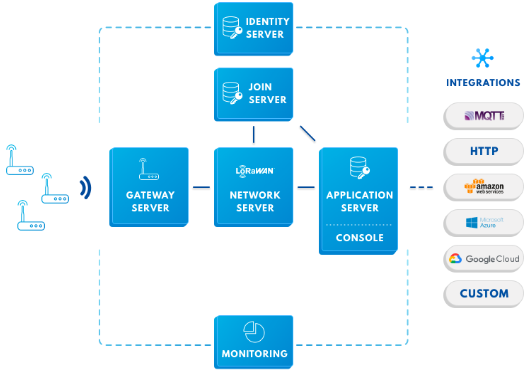
\includegraphics[width=\textwidth]{./Figuras/arquitectura_TTN.png}
	\caption{Diagrama en bloques de la red LoRaWAN a utilizar y sus posibles integraciones con terceras partes.}
	\label{fig:diagBloquesLoRaWAN}
\end{figure}

Esta integración se logrará a través de APIs HTTP o mediante suscripciones a tópicos de agentes de mensajería.\\
Los BES privados a desarrollar en este proyecto serán 3:
\begin{enumerate}
	\item Servicio de Recuperación de Datos: encargado de recuperar los datos enviados por los nodos a traves de la API proporcionada por la red LoRaWAN y almacenarlos en una base de datos.
	\item Base de datos (DB): encargado de almacenar los valores históricos de los nodos sensores y generar diferentes métricas para los reportes de estado.
	\item Interfaz Gráfica de Usuario (GUI): encargada de presentar el último estado recuperado de cada nodo al usuario final del sistema.
\end{enumerate}
%\end{consigna}


\section{Identificación y análisis de los interesados}
\label{sec:interesados}

\begin{consigna}{black} 

\begin{table}[H]
%\caption{Identificación de los interesados}
%\label{tab:interesados}
\begin{tabularx}{\linewidth}{@{}|l|X|X|l|@{}}
\hline
\rowcolor[HTML]{C0C0C0} 
Rol           & Nombre y Apellido & Organización 	& Puesto 	\\ \hline
Cliente    & \supname & \pertesupname & Docente investigador \\ \hline
\shortstack[l]{Responsable, auspiciante \\ e impulsor} & Ing. Milton E. Sosa & Universidad Nacional de Misiones & Egresado\\ \hline
Orientador    & \supname	      & \pertesupname 	& Docente investigador \\ \hline
Colaborador & Dr. Ing. Eduardo O. Sosa  &Universidad Nacional de Misiones &Docente Investigador    	\\ \hline
Colaborador & Ing. Germán A. Xánder     &Universidad Nacional de Misiones &Docente Investigador    	\\ \hline
\end{tabularx}
\end{table}
 
\begin{itemize}
	\item Ing. Marcelo E. Romeo, de vasta experiencia profesional en el ámbito de la microelectrónica e investigación y desarrollo para diferentes entidades y universidades nacionales.
	\item Dr. Ing. Eduardo O. Sosa, cuenta con más de 20 años de experiencia en el área de las TELCO, ex miembro colaborador de la RIU, profesor titular de la cátedra de Física en la Universidad Nacional de Misiones y lidera proyectos bilaterales entre Argentina y Alemania en el ámbito de WSN.
\end{itemize}
\end{consigna}

\section{1. Propósito del proyecto}
\label{sec:proposito}

\begin{consigna}{black}
El propósito de este proyecto es desarrollar un sistema formado por un circuito electrónico autónomo y un conjunto de software dedicado a la recuperación y almacenamiento de datos generados y transmitidos por el circuito.\\

El sistema debe ser capaz de permitir a las actuales redes de distribución de energía eléctrica reportar su estado actual de operación a un centro de monitoreo.
\end{consigna}

\section{2. Alcance del proyecto}
\label{sec:alcance}

\begin{consigna}{black}
Se pretende desarrollar un prototipo de HW capaz de ser autosuficiente en cuanto a la conversión, acumulación y gestión de energía eléctrica con el objeto de alimentar y permitir su operación en estado autónomo y permanente. Para ello se desarrollará un circuito de \textit{micro energy harvesting} basado en rectificadores de bajas pérdidas, acumuladores aptos para la aplicación final y un conversor DC/DC de alta eficiencia.\\

Se desarrollará una etapa de medición de valor eficaz de corriente alterna, con el objeto de medir la intensidad de corriente que actualmente circula por el conductor conectado a la salida de baja tensión e inmediatamente después del fusible aéreo de protección.\\

Agregado a los módulos mencionados anteriormente, un microcontrolador se encargará de la gestión de energía de todo el HW y de digitalizar todas las mediciones realizadas para finalmente, enviarlas al centro de operaciones a través de un módulo de comunicación.\\

Los BES se albergarán en una computadora de bajo costo que proporcionará suficientes recursos para su operación y ensayo en la etapa de desarollo.\\

No es parte del alcance del presente proyecto llegar a una etapa de lanzamiento del producto a clientes finales, sino la de lograr un demostrador tecnológico. Sin embargo, si los tiempos lo permiten y se logra contar con una infraestructura adecuada, se desean realizar ensayos \textit{end-to-end} en laboratorio sobre el sistema, involucrando los prototipos de hardware que fueran desarrollados, y una integración mínima entre los BES y la red LoRaWAN ya existente.\\
\end{consigna}

\section{3. Supuestos del proyecto}
\label{sec:supuestos}
\begin{consigna}{black}
Para el desarrollo del presente proyecto se supone que:
\begin{itemize}
	\item El autor del trabajo no tendrá ningún problema para hacerse de los insumos necesarios para alcanzar los objetivos recurriendo a distribuidores de componentes en el mercado local.
	\item Al momento de ensayar el sistema se contará con conectividad a internet.
	\item El responsable no tendrá en ningún momento limitaciones de movilidad.
	\item En caso de ser necesario realizar ensayos \textit{end-to-end}, el responsable deberá fabricar un banco de ensayos apropiado para simular los casos de uso y probar el sistema en su conjunto, como así disponer de instrumentos patrones para contrastar y verificar el correcto funcionamiento.
	\item Los ensayos \textit{end-to-end} no demorarán la fecha de finalización del proyecto.
\end{itemize}
\end{consigna}





\section{4. Requerimientos}
\label{sec:requerimientos}
%\begin{consigna}{black}
\begin{enumerate}
\item Grupo de requerimientos asociados con hardware
	\begin{enumerate}
	\item El dispositivo deberá ser de tipo \textit{plug and play}.
	\item El circuito impreso no deberá ocupar un volumen mayor a 10x10x5 cm.
	\item Basarse en un microcontrolador ESP32 y disponer de:
	\begin{itemize}
		\item 4 entradas analógicas.
		\item 3 salidas digitales.
		\item Unidad UART.
		\item Integrar un módulo de comunicaciones LoRa.
	\end{itemize}
	\item Deberá tener al menos 12 horas de autonomía de funcionamiento.
	\item Bajo consumo en modo ocioso: el consumo del hardware en total, no deberá superar los 5 mA cuando no está midiendo ni transmitiendo.
	\item El circuito elevador de tensión DC-DC deberá:
	\begin{itemize}
		\item Funcionar con tensiones menores a 2V en la entrada.
		\item Otorgar 5 Volts a la salida.
		\item Ser capaz de otorgar 300 miliamperes a la salida.
	\end{itemize}
	\item El transformador de corriente debe:
	\begin{itemize}
		\item Ser de tipo núcleo partido.
		\item Admitir 100 Amperes de corriente en el circuito primario y un máximo 5 Amperes en el circuito secundario.
	\end{itemize}
	\item \label{req_relay} El relay encargado de cambiar el modo de operación debe:
	\begin{itemize}
		\item Ser de tipo doble invesor sin retención.
		\item Su bobina debe poder energizarse con 5V o menos.
		\item Soportar al menos 5 Amperes de corriente por los contactos.
	\end{itemize} 
	\item Debe funcionar de manera independiente a la frecuencia de operación de la red 50/60 Hz.
	\item Debe funcionar de manera independiente a la tensión de fase del sistema de distribución 110/220 Voltios.
	\end{enumerate}
	
\item Grupo de requerimientos asociados con el firmware
	\begin{enumerate}
	\item Debe manejar un módulo de comunicación LoRa y protocolo LoRaWAN.
	\item Deberá tener un porcentaje de cobertura de tests unitarios del 60\% como mínimo.
	\item Antes configurarse en modo ocioso, debe desenergizar la etapa de medición de corriente y el módulo de comunicaciones con el objeto de ahorrar energía.
	\end{enumerate}
	
\item Grupo de requerimientos asociados con los BES
	\begin{enumerate}
		\item Todos los servicios deben poder correr en una Raspberry Pi 3.
		\item El software de los BES se desarrollará en lenguaje Python.
		\item Recuperar los datos de la red LoRaWAN.
		\item Almacenar los datos en una tabla de MySQL.
		\item GUI basada en Grafana.
	\end{enumerate}

\item Grupo de requerimientos asociados con ensayos de integración y \textit{end-to-end}
	\begin{enumerate}
		\item El banco de ensayos de hardware debe contar con una carga fantasma de al menos 10 Amperes y permitir realizar interrupciones de corriente de manera programada mediante una computadora adicional tipo Raspberry Pi o de manera manual.
		\item Los BES deben estar operativos al momento de realizar los ensayos.
		\item Contar con un gateway de acceso a una red LoRaWAN como por ejemplo \textit{The Things Network}.
	\end{enumerate}
\end{enumerate}
%\end{consigna}

\section{5. Entregables principales del proyecto}
\label{sec:entregables}
%\begin{consigna}{black}
\begin{itemize}
\item Diagrama esquemático
\item Lista de materiales
\item Código fuente del firmware
\item Diagrama de instalación
\item Informe final
\end{itemize}

%\end{consigna}

\section{6. Desglose del trabajo en tareas}
\label{sec:wbs}
%\begin{consigna}{black}
\begin{enumerate}
\item Grupo de tareas asociadas a planificación (Total: 35 hs)
	\begin{enumerate}
		\item Diseño de la arquitectura global del proyecto. (15 hs)
		\item Documentación del plan de proyecto. (20 hs)
	\end{enumerate}
\item Grupo de tareas asociadas al hardware (Total: 300 hs)
	\begin{enumerate}
		 \item Transductor de corriente. (Total: 16 hs)
			 \begin{enumerate}
			 	\item Análisis de transductores aptos para el hardware a desarrollar. (5 hs)
			 	\item Selección de componentes. (3 hs)
			 	\item Ensayo y evaluación del transductor de manera individual. (4 hs)
			 	\item Documentación de resultados del ensayo del transductor. (4 hs)
			 \end{enumerate}
			
		 \item Etapa de circuito de selección. (Total: 24 hs)
			 \begin{enumerate}
			 	\item Análisis de alternativas disponibles en el mercado. (10 hs)
			 	\item Selección de relays aptos en base a los requerimientos: tensión de bobina de 5 Volts y 5 Amperes de corriente. (6 hs)
			 	\item Ensayo del circuito de selección de manera individual. (4 hs)
			 	\item Documentación de ensayo. (4 hs)
			 \end{enumerate}			
			
		 \item Etapa de rectificación y filtrado. (Total: 49 hs)
			 \begin{enumerate}
				\item Análisis comparativo de alternativas para técnicas de rectificacion. (30 hs)
				\item Selección de componentes encargados de la etapa de rectificación. (10 hs)
				\item Ensayo de la etapa de rectificación de manera individual. (5 hs)
				\item Documentación de ensayos. (4 hs)
			 \end{enumerate}
			
		 \item Etapa de acumulación de energía. (Total: 35 hs)
			 \begin{enumerate}
			 	\item Análisis comparativo y selección de alternativas viables acorde al requerimiento de autonomía de operación. (10 hs)
			 	\item Ensayo de carga y descarga del acumulador de manera individual. (10 hs)
			 	\item Evaluación de resultados y estimación de la autonomía de operación en función de diferentes perfiles de consumo. (10 hs)
			 	\item Documentación ensayos. (5 hs)
			 \end{enumerate}
			 
		 \item Etapa de elevación de tensión. (Total: 20 hs)
			 \begin{enumerate}
			 	\item Análisis de alternativas técnicas para elevación de tensión aptas para el hardware a desarrollar. (15 hs)
			 	\item Ensayo y evaluación de la etapa de elevación de tensión de manera individual. (5 hs)
			 \end{enumerate}

		 \item Etapa de medición de corriente. (Total: 34 hs)
			 \begin{enumerate}
			 	\item Análisis comparativo y selección de un ciruito integrado dedicado a realizar la medición del valor eficaz de corriente. (20 hs)
			 	\item Ensayo y evaluación de la etapa de medición de valor eficaz de manera individual. (10 hs)
			 	\item Documentación de ensayos. (4 hs)
			 \end{enumerate}
			 
		 \item Etapa de acondicionamiento de señal posterior a la medición de corriente. (Total: 13 hs)
			 \begin{enumerate}
			 	\item Análisis de alternativas técnicas para filtrado y amplificación. (4 hs)
			 	\item Selección de componentes. (2 hs)
			 	\item Ensayo y evaluación de la etapa de filtrado y amplificación de manera individual. (4 hs)
			 	\item Documentación de ensayos. (3 hs)
			 \end{enumerate}
			 
		 \item Microcontrolador y módulo de comunicaciones. (Total: 50 hs)
			 \begin{enumerate}
			 	\item Análisis y selección de microcontroladores y módulos de comunicaciónes aptos para la aplicación. (30 hs)
			 	\item Pruebas de laboratorio del microcontrolador y módulo de comunicaciónes de manera individual. (20 hs)
			 \end{enumerate}
		
		 \item Circuito impreso. (Total: 59 hs)
			 \begin{enumerate}
			 	\item Ruteo del circuito impreso. (40 hs)
			 	\item Inspección. (6 hs)
			 	\item Montaje y soldado de componentes. (8 hs)
			 	\item Prueba y depuración. (5 hs)
			 \end{enumerate}			 			 			 
		\end{enumerate}

	\item Grupo de tareas asociadas al software (Total: 271 hs)
	\begin{enumerate}
		\item Tareas asociadas al firmware del microcontrolador (Total: 110 hs)
			\begin{enumerate}
				\item Definición de la "lógica de negocio" que regirá la operación del hardware a instalar \textit{in-situ}. (10 hs)
				\item Prototipado del firmware. (60 hs)
				\item Depuración de errores. (20 hs)
				\item Pruebas unitarias. (20 hs)
			\end{enumerate}
		
		 \item Tareas asociadas a los BES (Total: 96 hs)
			\begin{enumerate}
				\item Diseño de la arquitectura y lógica de operación de cada servicio. (14 hs)
				\item Instalación de los servicios. (30 hs)
				\item Creación de tablas en base de datos para el almacenamiento de valores históricos. (4 hs)
				\item Desarrollo del software encargado de recuperar los datos de la red LoRaWAN y almacenar en la base de datos. (20 hs)
				\item Desarrollo de la interfaz gráfica en Grafana. (8 hs)
				\item Pruebas de integración. (15 hs)
				\item Depuración de errores. (5 hs)
			\end{enumerate}
		\end{enumerate}
		
	\item Grupo de tareas asociadas a pruebas \textit{end-to-end}. (Total: 65 hs)
		\begin{enumerate}
		 	\item Definición de los casos de ensayo. (20 hs)
		 	\item Desarrollo del software. (20 hs)
		 	\item Ejecución de las pruebas. (15 hs)
		 	\item Depuración de errores. (10 hs)
		\end{enumerate}		
	\end{enumerate}

Cantidad total de horas: (671 hs)

%\end{consigna}

\section{7. Diagrama de Activity On Node}
\label{sec:AoN}

\begin{consigna}{red}
Armar el AoN a partir del WBS definido en la etapa anterior. 

%La figura \ref{fig:AoN} fue elaborada con el paquete latex tikz y pueden consultar la siguiente referencia \textit{online}:

%\url{https://www.overleaf.com/learn/latex/LaTeX_Graphics_using_TikZ:_A_Tutorial_for_Beginners_(Part_3)\%E2\%80\%94Creating_Flowcharts}

\end{consigna}

\begin{figure}[htpb]
\centering 
\includegraphics[width=.8\textwidth]{./Figuras/AoN.png}
\caption{Diagrama en \textit{Activity on Node}}
\label{fig:AoN}
\end{figure}

Indicar claramente en qué unidades están expresados los tiempos.
De ser necesario indicar los caminos semicríticos y analizar sus tiempos mediante un cuadro.
Es recomendable usar colores y un cuadro indicativo describiendo qué representa cada color, como se muestra en el siguiente ejemplo:



\section{8. Diagrama de Gantt}
\label{sec:gantt}

\begin{consigna}{red}
Utilizar el software Gantter for Google Drive o alguno similar para dibujar el diagrama de Gantt.

Existen muchos programas y recursos \textit{online} para hacer diagramas de gantt, entre las cuales destacamos:

\begin{itemize}
\item Planner
\item GanttProject
\item Trello + \textit{plugins}. En el siguiente link hay un tutorial oficial: \\ \url{https://blog.trello.com/es/diagrama-de-gantt-de-un-proyecto}
\item Creately, herramienta online colaborativa. \\\url{https://creately.com/diagram/example/ieb3p3ml/LaTeX}
\item Se puede hacer en latex con el paquete \textit{pgfgantt}\\ \url{http://ctan.dcc.uchile.cl/graphics/pgf/contrib/pgfgantt/pgfgantt.pdf}
\end{itemize}

Pegar acá una captura de pantalla del diagrama de Gantt, cuidando que la letra sea suficientemente grande como para ser legible. 
Si el diagrama queda demasiado ancho, se puede pegar primero la ``tabla'' del Gantt y luego pegar la parte del diagrama de barras del diagrama de Gantt.

Configurar el software para que en la parte de la tabla muestre los códigos del EDT (WBS).\\
Configurar el software para que al lado de cada barra muestre el nombre de cada tarea.\\
Revisar que la fecha de finalización coincida con lo indicado en el Acta Constitutiva.

En la figura \ref{fig:gantt}, se muestra un ejemplo de diagrama de gantt realizado con el paquete de \textit{pgfgantt}. En la plantilla pueden ver el código que lo genera y usarlo de base para construir el propio.

\begin{figure}[htbp]
\begin{center}
\begin{ganttchart}{1}{12}
  \gantttitle{2020}{12} \\
  \gantttitlelist{1,...,12}{1} \\
  \ganttgroup{Group 1}{1}{7} \\
  \ganttbar{Task 1}{1}{2} \\
  \ganttlinkedbar{Task 2}{3}{7} \ganttnewline
  \ganttmilestone{Milestone o hito}{7} \ganttnewline
  \ganttbar{Final Task}{8}{12}
  \ganttlink{elem2}{elem3}
  \ganttlink{elem3}{elem4}
\end{ganttchart}
\end{center}
\caption{Diagrama de gantt de ejemplo}
\label{fig:gantt}
\end{figure}

\end{consigna}

\section{9. Matriz de uso de recursos de materiales}
\label{sec:recursos}


\begin{table}[htpb]
\label{tab:recursos}
\centering
\begin{tabularx}{\linewidth}{@{}|c|X|X|X|X|X|@{}}
\hline
\cellcolor[HTML]{C0C0C0} & \cellcolor[HTML]{C0C0C0} & \multicolumn{4}{c|}{\cellcolor[HTML]{C0C0C0}Recursos requeridos (horas)} \\ \cline{3-6} 
\multirow{-2}{*}{\cellcolor[HTML]{C0C0C0}\begin{tabular}[c]{@{}c@{}}Código\\ WBS\end{tabular}} & \multirow{-2}{*}{\cellcolor[HTML]{C0C0C0}\begin{tabular}[c]{@{}c@{}}Nombre \\ tarea\end{tabular}} & Material 1 & Material 2 & Material 3 & Material 4 \\ \hline
 &  &  &  &  &  \\ \hline
 &  &  &  &  &  \\ \hline
 &  &  &  &  &  \\ \hline
 &  &  &  &  &  \\ \hline
\end{tabularx}%
\end{table}


\section{10. Presupuesto detallado del proyecto}
\label{sec:presupuesto}

\begin{consigna}{red}
Si el proyecto es complejo entonces separarlo en partes:
\begin{itemize}
\item Un total global, indicando el subtotal acumulado por cada una de las áreas.
\item El desglose detallado del subtotal de cada una de las áreas.
\end{itemize}

IMPORTANTE: No olvidarse de considerar los COSTOS INDIRECTOS.

\end{consigna}

\begin{table}[htpb]
\centering
\begin{tabularx}{\linewidth}{@{}|X|c|r|r|@{}}
\hline
\rowcolor[HTML]{C0C0C0} 
\multicolumn{4}{|c|}{\cellcolor[HTML]{C0C0C0}COSTOS DIRECTOS} \\ \hline
\rowcolor[HTML]{C0C0C0} 
Descripción &
  \multicolumn{1}{c|}{\cellcolor[HTML]{C0C0C0}Cantidad} &
  \multicolumn{1}{c|}{\cellcolor[HTML]{C0C0C0}Valor unitario} &
  \multicolumn{1}{c|}{\cellcolor[HTML]{C0C0C0}Valor total} \\ \hline
 &
  \multicolumn{1}{c|}{} &
  \multicolumn{1}{c|}{} &
  \multicolumn{1}{c|}{} \\ \hline
 &
  \multicolumn{1}{c|}{} &
  \multicolumn{1}{c|}{} &
  \multicolumn{1}{c|}{} \\ \hline
\multicolumn{1}{|l|}{} &
   &
   &
   \\ \hline
\multicolumn{1}{|l|}{} &
   &
   &
   \\ \hline
\multicolumn{3}{|c|}{SUBTOTAL} &
  \multicolumn{1}{c|}{} \\ \hline
\rowcolor[HTML]{C0C0C0} 
\multicolumn{4}{|c|}{\cellcolor[HTML]{C0C0C0}COSTOS INDIRECTOS} \\ \hline
\rowcolor[HTML]{C0C0C0} 
Descripción &
  \multicolumn{1}{c|}{\cellcolor[HTML]{C0C0C0}Cantidad} &
  \multicolumn{1}{c|}{\cellcolor[HTML]{C0C0C0}Valor unitario} &
  \multicolumn{1}{c|}{\cellcolor[HTML]{C0C0C0}Valor total} \\ \hline
\multicolumn{1}{|l|}{} &
   &
   &
   \\ \hline
\multicolumn{1}{|l|}{} &
   &
   &
   \\ \hline
\multicolumn{1}{|l|}{} &
   &
   &
   \\ \hline
\multicolumn{3}{|c|}{SUBTOTAL} &
  \multicolumn{1}{c|}{} \\ \hline
\rowcolor[HTML]{C0C0C0}
\multicolumn{3}{|c|}{TOTAL} &
   \\ \hline
\end{tabularx}%
\end{table}


\section{11. Matriz de asignación de responsabilidades}
\label{sec:responsabilidades}
\begin{consigna}{red}
Establecer la matriz de asignación de responsabilidades y el manejo de la autoridad completando la siguiente tabla:

\begin{table}[htpb]
\centering
\resizebox{\textwidth}{!}{%
\begin{tabular}{|c|c|c|c|c|c|}
\hline
\rowcolor[HTML]{C0C0C0} 
\cellcolor[HTML]{C0C0C0} &
  \cellcolor[HTML]{C0C0C0} &
  \multicolumn{4}{c|}{\cellcolor[HTML]{C0C0C0}Listar todos los nombres y roles del proyecto} \\ \cline{3-6} 
\rowcolor[HTML]{C0C0C0} 
\cellcolor[HTML]{C0C0C0} &
  \cellcolor[HTML]{C0C0C0} &
  Responsable &
  Orientador &
  Equipo &
  Cliente \\ \cline{3-6} 
\rowcolor[HTML]{C0C0C0} 
\multirow{-3}{*}{\cellcolor[HTML]{C0C0C0}\begin{tabular}[c]{@{}c@{}}Código\\ WBS\end{tabular}} &
  \multirow{-3}{*}{\cellcolor[HTML]{C0C0C0}Nombre de la tarea} &
  \authorname &
  \supname &
  Nombre de alguien &
  \clientename \\ \hline
 &  &  &  &  &  \\ \hline
 &  &  &  &  &  \\ \hline
 &  &  &  &  &  \\ \hline
\end{tabular}%
}
\end{table}

{\footnotesize
Referencias:
\begin{itemize}
	\item P = Responsabilidad Primaria
	\item S = Responsabilidad Secundaria
	\item A = Aprobación
	\item I = Informado
	\item C = Consultado
\end{itemize}
} %footnotesize

Una de las columnas debe ser para el Director, ya que se supone que participará en el proyecto.
A su vez se debe cuidar que no queden muchas tareas seguidas sin ``A'' o ``I''.

Importante: es redundante poner ``I/A'' o ``I/C'', porque para aprobarlo o responder consultas primero la persona debe ser informada.

\end{consigna}

\section{12. Gestión de riesgos}
\label{sec:riesgos}

\begin{consigna}{red}
a) Identificación de los riesgos (al menos cinco) y estimación de sus consecuencias:
 
Riesgo 1: detallar el riesgo (riesgo es algo que si ocurre altera los planes previstos)
\begin{itemize}
\item Severidad (S): mientras más severo, más alto es el número (usar números del 1 al 10).\\
Justificar el motivo por el cual se asigna determinado número de severidad (S).
\item Probabilidad de ocurrencia (O): mientras más probable, más alto es el número (usar del 1 al 10).\\
Justificar el motivo por el cual se asigna determinado número de (O). 
\end{itemize}   

Riesgo 2:
\begin{itemize}
\item Severidad (S): 
\item Ocurrencia (O):
\end{itemize}

Riesgo 3:
\begin{itemize}
\item Severidad (S): 
\item Ocurrencia (O):
\end{itemize}


b) Tabla de gestión de riesgos:      (El RPN se calcula como RPN=SxO)

\begin{table}[htpb]
\centering
\begin{tabularx}{\linewidth}{@{}|X|c|c|c|c|c|c|@{}}
\hline
\rowcolor[HTML]{C0C0C0} 
Riesgo & S & O & RPN & S* & O* & RPN* \\ \hline
       &   &   &     &    &    &      \\ \hline
       &   &   &     &    &    &      \\ \hline
       &   &   &     &    &    &      \\ \hline
       &   &   &     &    &    &      \\ \hline
       &   &   &     &    &    &      \\ \hline
\end{tabularx}%
\end{table}

Criterio adoptado: 
Se tomarán medidas de mitigación en los riesgos cuyos números de RPN sean mayores a ....

Nota: los valores marcados con (*) en la tabla corresponden luego de haber aplicado la mitigación.

c) Plan de mitigación de los riesgos que originalmente excedían el RPN máximo establecido:
 
Riesgo 1: Plan de mitigación (si por el RPN fuera necesario elaborar un plan de mitigación).
  Nueva asignación de S y O, con su respectiva justificación:
  - Severidad (S): mientras más severo, más alto es el número (usar números del 1 al 10).
          Justificar el motivo por el cual se asigna determinado número de severidad (S).
  - Probabilidad de ocurrencia (O): mientras más probable, más alto es el número (usar del 1 al 10).
          Justificar el motivo por el cual se asigna determinado número de (O).

Riesgo 2: Plan de mitigación (si por el RPN fuera necesario elaborar un plan de mitigación).
 
Riesgo 3: Plan de mitigación (si por el RPN fuera necesario elaborar un plan de mitigación)

\end{consigna}


\section{13. Gestión de la calidad}
\label{sec:calidad}

\begin{consigna}{red}
Para cada uno de los requerimientos del proyecto indique:
\begin{itemize} 
\item Req \#1: Copiar acá el requerimiento.

Verificación y validación:

\begin{itemize}
\item Verificación para confirmar si se cumplió con lo requerido antes de mostrar el sistema al cliente:\\
Detallar 
\item Validación con el cliente para confirmar que está de acuerdo en que se cumplió con lo requerido:\\
Detallar  
\end{itemize}

\end{itemize}

Tener en cuenta que en este contexto se pueden mencionar simulaciones, cálculos, revisión de hojas de datos, consulta con expertos, etc.

\end{consigna}

\section{14. Comunicación del proyecto}
\label{sec:comunicaciones}

\begin{consigna}{red}
El plan de comunicación del proyecto es el siguiente:
\end{consigna}

% Please add the following required packages to your document preamble:
% \usepackage{graphicx}
% \usepackage[table,xcdraw]{xcolor}
% If you use beamer only pass "xcolor=table" option, i.e. \documentclass[xcolor=table]{beamer}
\begin{table}[htpb]
\centering
\resizebox{\textwidth}{!}{%
\begin{tabular}{|c|c|c|c|c|c|}
\hline
\rowcolor[HTML]{C0C0C0} 
\multicolumn{6}{|c|}{\cellcolor[HTML]{C0C0C0}PLAN DE COMUNICACIÓN DEL PROYECTO}           \\ \hline
\rowcolor[HTML]{C0C0C0} 
¿Qué comunicar? & Audiencia & Propósito & Frecuencia & Método de comunicac. & Responsable \\ \hline
                &           &           &            &                      &             \\ \hline
                &           &           &            &                      &             \\ \hline
                &           &           &            &                      &             \\ \hline
                &           &           &            &                      &             \\ \hline
                &           &           &            &                      &             \\ \hline
\end{tabular}%
}
\end{table}

\section{15. Gestión de Compras}
\label{sec:compras}

\begin{consigna}{red}
En caso de tener que comprar elementos o contratar servicios:
a) Explique con qué criterios elegiría a un proveedor.
b) Redacte el Statement of Work correspondiente.
\end{consigna}

\section{16. Seguimiento y control}
\label{sec:seguimiento}

\begin{consigna}{red}
Para cada tarea del proyecto establecer la frecuencia y los indicadores con los se seguirá su avance y quién será el responsable de hacer dicho seguimiento y a quién debe comunicarse la situación (en concordancia con el Plan de Comunicación del proyecto).

El indicador de avance tiene que ser algo medible, mejor incluso si se puede medir en \% de avance. Por ejemplo,se pueden indicar en esta columna cosas como ``cantidad de conexiones ruteadeas'' o ``cantidad de funciones implementadas'', pero no algo genérico y ambiguo como ``\%'', porque el lector no sabe porcentaje de qué cosa.

\end{consigna}

\begin{table}[!htpb]
\centering
\begin{tabularx}{\linewidth}{@{}|X|X|X|X|X|X|@{}}
\hline
\rowcolor[HTML]{C0C0C0} 
\multicolumn{6}{|c|}{\cellcolor[HTML]{C0C0C0}SEGUIMIENTO DE AVANCE}                                                                       \\ \hline
\rowcolor[HTML]{C0C0C0} 
Tarea del WBS & Indicador de avance & Frecuencia de reporte & Resp. de seguimiento & Persona a ser informada & Método de comunic. \\ \hline
 &  &  &  &  &  \\ \hline
 &  &  &  &  &  \\ \hline
 &  &  &  &  &  \\ \hline
 &  &  &  &  &  \\ \hline
 &  &  &  &  &  \\ \hline
\end{tabularx}%
%}
\end{table}

\section{17. Procesos de cierre}    
\label{sec:cierre}

\begin{consigna}{red}
Establecer las pautas de trabajo para realizar una reunión final de evaluación del proyecto, tal que contemple las siguientes actividades:

\begin{itemize}
\item Pautas de trabajo que se seguirán para analizar si se respetó el Plan de Proyecto original:
 - Indicar quién se ocupará de hacer esto y cuál será el procedimiento a aplicar. 
\item Identificación de las técnicas y procedimientos útiles e inútiles que se utilizaron, y los problemas que surgieron y cómo se solucionaron:
 - Indicar quién se ocupará de hacer esto y cuál será el procedimiento para dejar registro.
\item Indicar quién organizará el acto de agradecimiento a todos los interesados, y en especial al equipo de trabajo y colaboradores:
  - Indicar esto y quién financiará los gastos correspondientes.
\end{itemize}

\end{consigna}


\end{document}
